\documentclass{guide}

\title{Knopjes, LEDs en Weerstand}
\level{1}

\begin{document}
\section{LEDs}
Voor het CSN miniproject moet je een aantal LEDs gaan aansturen met de Raspberry Pi. Deze zijn (gratis) te verkrijgen in de TI Labwinkel. LEDs komen in verschillende kleuren: Rood, Geel, Groen, Blauw en Wit (de zwarte LEDs geven onzichtbaar infrarood licht). Een LED kan worden aangestuurd met gelijkspanning zoals uit je Raspberry Pi. Let er daarbij op dat lange pin / ronde kant op de VCC (+3,3V of +5V) moet worden aangesloten, en de korte pin / afgeplatte kant op de ground moet (0V).

\begin{figure}[h]
  \centering
  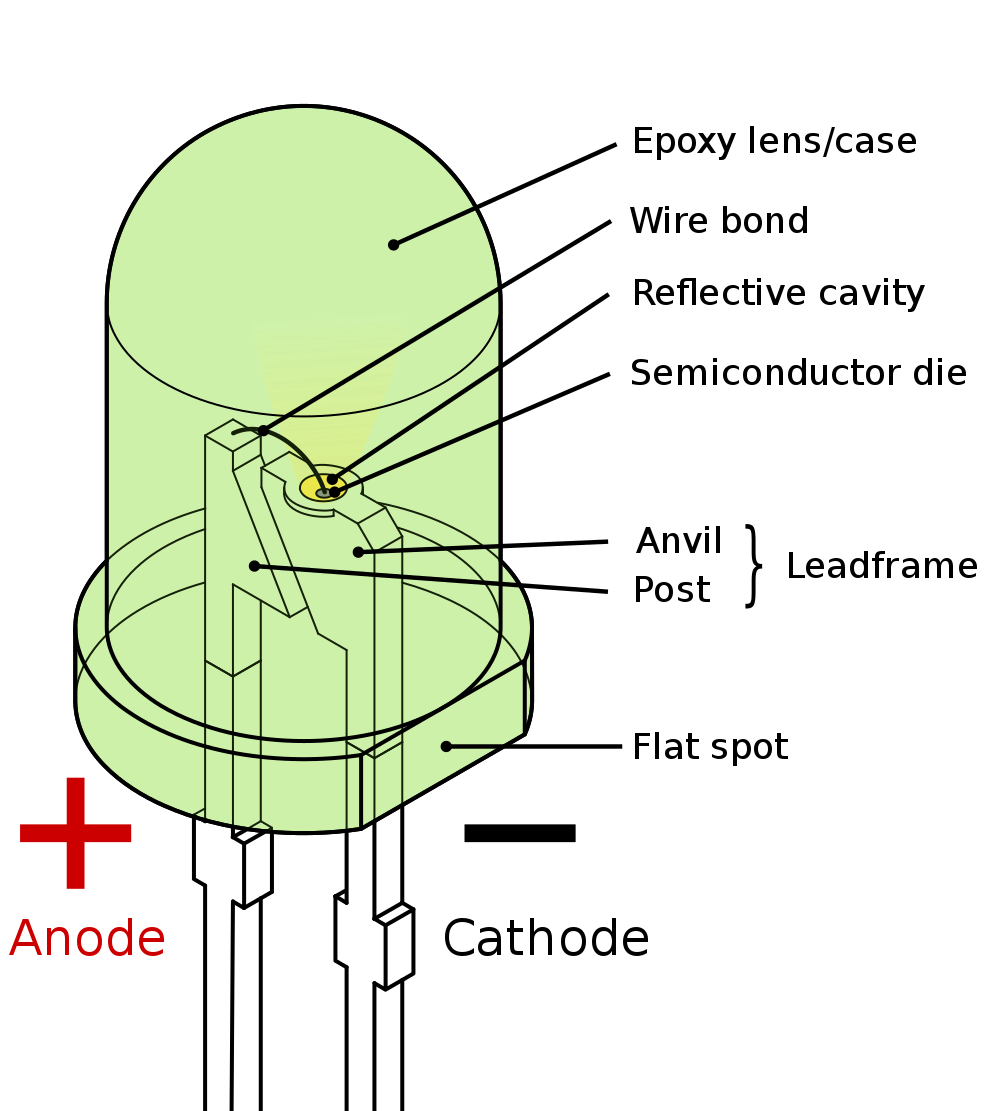
\includegraphics[width=4cm]{images/led.png}
  \caption{Schematische weergave van een LED (bron: \href{https://upload.wikimedia.org/wikipedia/commons/thumb/f/f9/LED\%2C_5mm\%2C_green_\%28en\%29.svg/1000px-LED\%2C_5mm\%2C_green_\%28en\%29.svg.png}{Wikipedia}).} \label{fig:led}
\end{figure}

\section{Knopjes}
Naast LEDs zul je ook knopjes nodig hebben. Ook deze zijn gratis bij de TI Labwinkel te halen. De knopjes die we gebruiken hebben vier pinnen, waarvan er steeds twee aan elkaar gekoppeld zijn. Effectief hebben we dus maar met twee pinnen te maken. De paren van tegenoverliggende pinnen zijn telkens aan elkaar verbonden, en als je op de knop drukt wordt stroom van links naar rechts (of vice versa) doorgegeven. De knop kan over de richel in het midden van een breadboard heen worden gezet.

\begin{figure}[h]
  \centering
  \vspace{3mm}
  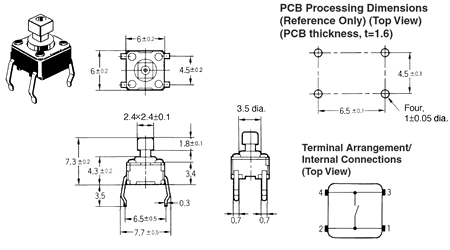
\includegraphics[width=0.6\textwidth]{images/button.png}
  \caption{Schematische tekening van de knopjes (bron: \href{https://www.google.com/url?sa=i&rct=j&q=&esrc=s&source=images&cd=&cad=rja&uact=8&ved=2ahUKEwiJ387Z9MndAhUO6qQKHafLD_kQjRx6BAgBEAU&url=https\%3A\%2F\%2Fecb.omron.com.sg\%2Fproduct-detail\%3FpartId\%3D460&psig=AOvVaw3-QL0EFgRXec_37ypIDQD0&ust=1537544210056281}{Omron}).} \label{fig:button}
\end{figure}

\section{Weerstand}
Om te voorkomen dat je LED uit elkaar spat moet je hier een weerstand tussen zetten. Weerstanden zijn gratis bij de TI Labwinkel te halen. Een weerstand beperkt de doorgang van elektrische stroom en vermindert hiermee het vermogen dat door de LED gaat. Weerstanden kunnen een hogere of lagere weerstandwaarde hebben, dit wordt gemeten in Ohm ($\Omega$). Een lage weerstandswaarde beperkt de stroomdoorgang minder dan een hoge weerstandwaarde. Koperen draadjes hebben een zeer lage weerstand, terwijl niet-geleidende materialen zoals glas of plastic een zeer hoge weerstand hebben. Voor een LED ligt de hoeveelheid weerstand af van de kleur, de stroombron, en de gewenste helderheid. In de praktijk is $1 k\Omega$ ($1000 \Omega$) in principe altijd goed.

\begin{figure}[h]
  \centering
  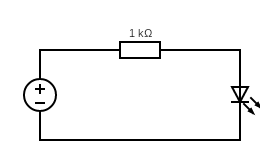
\includegraphics[width=3cm]{images/circuit.png}
  \caption{Een LED met een weerstand.} \label{fig:circuit}
\end{figure}

De LEDs in de TI Labshop zitten in gelabelde bakjes, maar ook zonder de labels is het mogelijk de verschillende weerstanden uit elkaar te houden. Een weerstand is namelijk voorzien van vier of vijf gekleurde banen. De eerste drie of vier geven de weerstand aan: de eerste twee zet je als cijfers achter elkaar (zie de tabel in Figuur~\ref{fig:resistors} voor de kleurcodes), en dit vermenigvuldig je met de derde (ook in de tabel). De laatste geeft aan hoeveel de daadwerkelijke weerstand ernaast kan zitten.

\section{Voor de aspirant-electrotechnicus}
Door een weerstand van $1 k\Omega$ te gebruiken voor een LED zit je in principe altijd goed: dit is namelijk meer dan strikt noodzakelijk, wat betekent dat je nooit teveel stroom door de LED stuurt en alleen wat helderheid verliest. Als je exact wilt weten welke weerstand je voor een LED (of ander onderdeel) nodig hebt, kun je de wet van Ohm gebruiken. Deze kan worden geschreven als $R = \frac{V}{I}$, waarbij R voor de gezochte weerstand staat, V voor het voltage staat (doorgaans 3,3V of 5V), en I voor de stroom in Amp\'{e}re.

Ieder elektrisch onderdeel heeft een eigen spanningsval ($V_f$), die aangeeft hoeveel spanning er aan weerstand van het onderdeel verloren gaat. Voor een rode, gele of geel-groene is dit $1,8V$, en voor een blauwe, groene of witte LED is dit $3,3V$. Door dit van het voltage van je spanningsbron af te trekken heb je de gewenste $V$ gevonden. Dit deel je door de ideale stroomsterkte voor een LED (meestal $25 mA$) om de minimale weerstand te vinden. De totale formule ziet er dus als volgt uit: $$R = \frac{V-V_f}{0,025A}$$

Het resultaat van deze berekening is hieronder in Tabel~\ref{tab:resistors} weergegeven. Let erop dat dit de minimale weerstand is, dus dat je naar boven moet afronden!
\begin{table}[h]
  \centering
  \begin{tabular}{|r|l|l|}
    \hline
    & Rood/geel/geel-groen & Blauw/groen/wit/UV \\
    \hline
    3,3V & $60 \Omega$ & $0 \Omega$ \\
    \hline
    5V & $128 \Omega$ & $68 \Omega$ \\
    \hline
  \end{tabular}
  \caption{Minimale weerstanden voor gebruikelijke LED-types en spanningsbronnen.}\label{tab:resistors}
\end{table}

\begin{figure}[p]
  \centering
  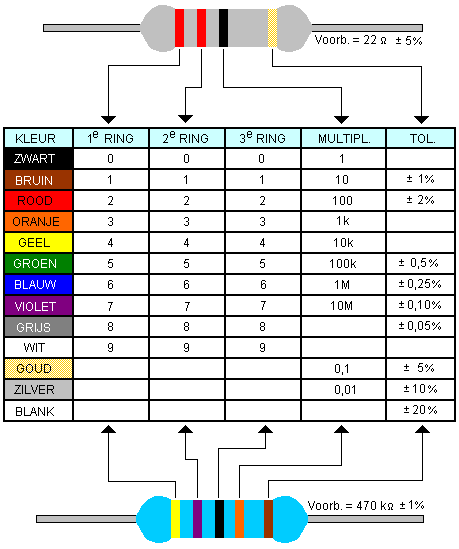
\includegraphics[width=0.6\textwidth]{images/resistors.png}
  \caption{De kleurcodering van weerstanden (bron: \href{https://a29.veron.nl/wp-content/uploads/2015/09/weerstandscodes.gif}{VERON}).} \label{fig:resistor}
\end{figure}

\end{document}
